\documentclass{article}
\usepackage{amsmath, amssymb, amsthm} 
\usepackage{xcolor} % For color usage
\usepackage{geometry}
\geometry{a4paper, margin=1in, top=1in}
\usepackage{fancyhdr}
\usepackage{tabularx}
\usepackage{titlesec}
\usepackage{titling}
\usepackage{graphicx}
\usepackage{bbding}
\usepackage{hyperref}
\usepackage{bbding}

% Define the lemma environment
\theoremstyle{definition}
\newtheorem{lemma}{Lemma}

\renewcommand{\footnoterule}{
    \vspace*{1mm} % Space before the rule
    \hrule width \linewidth height 0.4pt % Rule specification
    \vspace*{2mm} % Space after the rule
}


\pagestyle{fancy}
\fancyhead[L]{Edric Ho}
\fancyfoot[C]{\thepage}


\setlength{\droptitle}{-2.5cm} % title position
\title{MAT240 Lecture Notes}
\author{Edric Ho}
\date{24' Fall Semester}

\begin{document}

% course logistics page
\begin{center}
    \vspace*{0.5cm} % Adjust vertical space to center the title on the page
    {\Huge \textbf{Course Logistics}} % Main title
    \vspace{0.4cm} % Space between title and the rest of the content
\end{center}

\begin{enumerate}
    \item \textbf{Instructor:} Prof. Gerbelli \qquad \textbf{email:} \texttt{m.gerbelli@utoronto.ca}
    
    \item \textbf{Lecture:} Tue 11:00 - 13:00, Thu 12:00 - 13:00 \qquad \textbf{Office Hours:} Tuesdays 2-4 PM, online
    
    \item \textbf{Assignments:} There will be 10 assignments, each worth 10 points (accumulatively \(n\) points in total).
    The total mark will be calculated by: 
    \[
    \text{Assignment Grade} = \min\left(100,\, \frac{n}{0.8} \times 100\right).
    \]
    
    \item \textbf{Term tests:}
    \begin{enumerate}
        \item \textbf{Term test 1:} Thursday, October $3^{rd}$, 12:10 - 1:00 PM
        \item \textbf{Term test 2:} Thursday, November $7^{th}$, 12:10 - 1:00 PM
    \end{enumerate}
    
    \item \textbf{Mark:} 
    \[
    \text{Max}\left(0.2a + 0.225t1 + 0.225t2 + 0.35f, 0.2a + 0.25 \max(t1, t2) + 0.10 \min(t1, t2) + 0.45f\right)
    \]
    
    \item \textbf{Lecture schedule and relative reading:}
\end{enumerate}

\begin{tabularx}{\textwidth} {
    | c 
    | >{\raggedright\arraybackslash}X 
    | >{\centering\arraybackslash}X 
    | >{\raggedleft\arraybackslash}X | }
    \hline
    \textbf{Week} & \textbf{Date} & \textbf{Topic} & \textbf{Reading} \\
    \hline
    1 & September 3 & Sets and Maps & Appendix A - B \\
    \hline
    \, & September 5 & $\mathbb{F}$, $\mathbb{C}$, Modular Arithmetic & Appendix C \\
    \hline
    2 & September 10 & Finite Fields & Notes on Finite Fields \\
    \hline
    \, & September 12 & Vector Spaces & 1.1 - 1.2 \\
    \hline
    3 & September 17 & Vector Spaces + Subspaces & 1.3 - 1.4 \\
    \hline
    \, & September 19 & Linear Relations + Dependence & 1.4 - 1.5 \\
    \hline
    4 & September 24 & Bases and Dimension (max LL subset, if time) & 1.6 - 1.7 \\
    \hline
    \, & September 26 & Review & \\
    \hline
    5 & October 1 & Linear Transformation & 2.1 \\
    \hline
    \, & October 3 & Midterm 1 & \\
    \hline
    6 & October 8 & Matrix of Linear Transformation & 2.2 \\
    \hline
    \, & October 10 & Composition & 2.3 \\
    \hline
    7 & October 15 & Invertibility and Isomorphisms & 2.4 \\
    \hline
    \, & October 17 & Dual Spaces & 2.6 \\
    \hline
    8 & October 22 & Change of Basis & 2.5 \\
    \hline
    \, & October 24 & Review & \\
    \hline
    9 & November 5 & Elementary Matrices & 3.1 \\
    \hline
    \, & November 7 & Midterm 2 & \\
    \hline
    10 & November 12 & Rank and Inverse & 3.2 \\
    \hline
    \, & November 14 & $2 \times 2$ Determinants & 4.1 \\
    \hline
    11 & November 19 & $n \times n$ Determinants & 4.2 \\
    \hline
    \, & November 21 & Properties of the Determinant & 4.3 \\
    \hline
    12 & November 26 & Characterization of the Determinant & 4.4 \\
    \hline
    \, & November 28 & Review & \\
    \hline
\end{tabularx}


% title
\maketitle

% lecture pages input
\section*{Lecture 1: Sets and Maps (Sep. $3^{rd}$)}

% SETS
\subsection*{\colorbox{yellow}{Sets.}}
\qquad A set is a collection of distinct elements. If an element \(x\) is in the set \(S\), we write \(x \in S\). If \(x\) is not, then we write \(x \notin S\).\\ 
\, \\
\textbf{Example:} $\mathbb{P} = \{ x \mid x \text{ is a prime number} \}$. From the set definition, we know that: \(5 \in \mathbb{P},\, 4 \notin \mathbb{P}\).\\

\begin{enumerate}
    \item \textbf{Some useful sets:} 
    \[
        \mathbb{R}: \text{ Reals},\quad \mathbb{Q}: \text{ Rationals},\quad \mathbb{Z}: \text{ Integers},\quad \mathbb{N}: \text{ Naturals}.
    \]
    \item \textbf{Describing a set:}
        \begin{itemize}
            \item Listing all of the elements in the set (Remark: Ordering in a set does not matter):
            \begin{itemize}
                \item \(A = \{1, 2, 3\} \qquad B = \{2, 0, -1\}\) 
            \end{itemize}
            \item Specifying the characteristics/properties:
            \begin{itemize}
                \item \(C = \{ n \in \mathbb{N} :\, 4 \mid n \}\)
            \end{itemize}
            \item The set with no elements is called the empty set, and it is \textbf{denoted as \(\varnothing\) instead of \{\}}.
        \end{itemize}
    \item \textbf{Subset:} If \(S, T\) are sets such that all elements of \(S\) are contained in \(T\), we say that \(S\) is a subset of \(T\) (we write \(S \subset T\)).
    \item \textbf{Sets equality:} Two sets contain exactly the same elements; we write \(S = T\). 
        \[ S = T \Leftrightarrow (S \subset T) \land (T \subset S)\]
    \item \textbf{Proper Subset:} If \(S \subset T\) but \(T \neq S\), then we say \(S\) is a proper subset of \(T\) and we write \(S \subsetneq T\).
        \[A \subsetneq B \Leftrightarrow \forall x \, (x \in A \implies x \in B) \land \exists x \, (x \notin A \land x \in B)\]
    \item \textbf{Operations on sets:} 
        \begin{itemize}
            \item \textbf{Union (\(\cup\)):} If \(S, T\) are sets, the union of \(S\) and \(T\) is:
                \[S \cup T = \{x \mid (x \in S) \lor (x \in T)\}\]
            \item \textbf{Intersection (\(\cap\)):} If \(S, T\) are sets, the intersection of \(S\) and \(T\) is:
                \[S \cap T = \{x \mid (x \in S) \land (x \in T)\}\]
            \item \textbf{Example:} Let \(\mathbf{N} = \{x \in \mathbb{Z} \mid x > 0\} = \{1, 2, 3, 4, \dots\}\) be the set of natural numbers, and let \(-\mathbf{N} = \{x \in \mathbb{Z} \mid x < 0\}\) be the set of negative integers. We can have the following operations:
                \[\mathbf{N} \cup -\mathbf{N} = \{x \in \mathbb{Z} \mid x \neq 0\}\]
                \[\mathbf{N} \cap -\mathbf{N} = \varnothing \quad \text{(Disjoint)}\] 
            \item \textbf{Union and Intersection over multiple sets:} If we have a list of sets \(S_1, S_2, \dots, S_k\), we can form their union and intersection using the following representations:
                \[\textbf{Union of all sets:}\quad\bigcup_{i=1}^{k} S_i = \{x \mid x \in S_i, \, \exists S_i, i = 1, \dots, k\}\]
                \[\textbf{Intersection of all sets:}\quad\bigcap_{i=1}^{k} S_i = \{x \mid x \in S_i, \, \forall i = 1, \dots, k\}\]
        \end{itemize}
\newpage
    \item \textbf{Relations on Sets:} A relation on a set \(A\) is a rule for determining whether, for any elements \(x\) and \(y\) in \(A\), \(x\) stands in a given relationship to \(y\).
        \begin{itemize}
            \item \textbf{Relation:} A relation on \(A\) is any set \(S\) of ordered pairs of elements of \(A\). The elements \(x\) and \(y\) satisfy the relation \textbf{iff} \((x, y) \in S\).
                \begin{itemize}
                    \item Example: \quad \(\forall x \in \mathbb{R}, \exists y \in \mathbb{R}, x \leq y\) \quad (The "greater than or equal to" relation in reals)
                \end{itemize}
            \item \textbf{Equivalence Relations:} A special type of relation, \(S\) is an \textbf{equivalence relation} on \(A\) if it satisfies:
                \begin{enumerate}
                    \item \textbf{Reflexivity:} \(\forall x \in A, \, x \sim x\)
                    \item \textbf{Symmetry:} \(x \sim y \implies y \sim x\)
                    \item \textbf{Transitivity:} \((x \sim y) \land (y \sim z) \implies x \sim z\)
                \end{enumerate}
                
                \subsubsection*{Example:}
                Has the same birthday relation: Consider a set \(A\) of people. Define a relation \(R\) on \(A\) such that for any two people \(a, b \in A\):
                \[
                a \, R \, b \text{ if and only if } a \text{ and } b \text{ have the same birthday}.
                \]
                \begin{itemize}
                    \item \textbf{Reflexive:} Every person has the same birthday as themselves, so \(a \, R \, a\) for all \(a \in A\).
                    \item \textbf{Symmetric:} If \(a \, R \, b\), then \(b \, R \, a\), since having the same birthday works both ways.
                    \item \textbf{Transitive:} If \(a \, R \, b\) and \(b \, R \, c\), then \(a \, R \, c\), since if \(a\) shares a birthday with \(b\) and \(b\) with \(c\), then \(a\) and \(c\) share the same birthday.
                \end{itemize}
                This ``has the same birthday" relation is an equivalence relation. The equivalence classes are groups of people who share the same birthday.

                \subsubsection*{Question:} 
                \qquad Provide an example of an equivalence relation.
        \end{itemize}
\end{enumerate}

\vspace*{- 0.1cm}


% FUNCTIONS
\subsection*{\colorbox{yellow}{Functions.}}
\qquad If S and T are sets, then a \textbf{function} $f$ from S to T, denoted \(f: \, S \rightarrow T\), is a rule assigning to each $x \in S$ an unique element $f(x)\in T$. 
    \begin{enumerate}
        %
        \item \textbf{Terminologies:}
            \begin{itemize}
                \item $f(x)$ is the \textbf{image of $x$ under $f$}.
                \item \(\forall x \in S \), \( x \) is called the \textbf{preimage of } \( f(x) \) \textbf{ under } \( f \).
                \item S is the \textbf{domain} of $f$, $T$ is the \textbf{codomain} of $f$, the \textbf{range of $f$} is the set:
                    \(\{f(x) \mid x \in S\} \subset T\)
                \item \textbf{Codomain:} of a function  $f: S \rightarrow T$  is the set  $T$  that includes all potential values the function could map to. It is specified when defining the function, but not every element in the codomain is necessarily an output of the function.
                \end{itemize}
        %
        \item \textbf{Image and Preimage of Subsets under a Function:}
                \begin{itemize}
                    \item If $U \subset S$ is a subset, then the image of $U$ is:
                        \[ f(U) = \{f(x) \mid x \in U\}\]
                    \item If $V \subset T$, then the preimage of $V$ is:
                        \[ f^{-1}(V) = \{x \mid f(x) \in V\}\]
                    \item If \( f: S \rightarrow T \) and \( U \subseteq S \), then the restriction of \( f \) to \( U \), denoted \( f|_U \), is defined by
                        \[ f|_U(x) = f(x) \quad \text{for all } x \in U. \]
                \end{itemize}
            \vspace{-0.8cm}
            \subsubsection*{Example.}
            \qquad Let $S = \{x \in \mathbb{R} \mid \, |x| \ge 1\}$ and let $f: S \rightarrow \mathbb{R}$ be the function sends $x$ to \(\frac{1}{x^{2}}\),
                \[f(x) = \frac{1}{x^{2}}\]
            \vspace*{-0.2cm}
            \begin{itemize}
                \item The domain is S, the codomain is $\mathbb{R}$, and the range is \((0,1]\).
                \item Since \( f(2) = \frac{1}{4} \), then \( \frac{1}{4} \) is the image of 2. \(-2\) is also the preimage of \( \frac{1}{4} \).
                \item The image of \([1, 10]\) is \(\left[ \frac{1}{100}, 1 \right]\) and the preimage of \((0, \frac{1}{2})\) is \((\sqrt{2}, \infty) \cup (-\infty, -\sqrt{2})\).
            \end{itemize}
            \vspace*{0.5cm}
        %
        \item \textbf{Types of functions:}
            \begin{itemize}
                \item \textbf{Injection (One-to-one):} If every element in the range has a unique preimage, we say $f$ is injective.
                \item \textbf{Surjection (Onto):} If every element in the codomain of $f$ is in the range of $f$, we say $f$ is surjective.
                \item \textbf{Bijection (One-to-one and Onto):} If $f$ is surjective and injective, we say $f$ is bijective.\\
                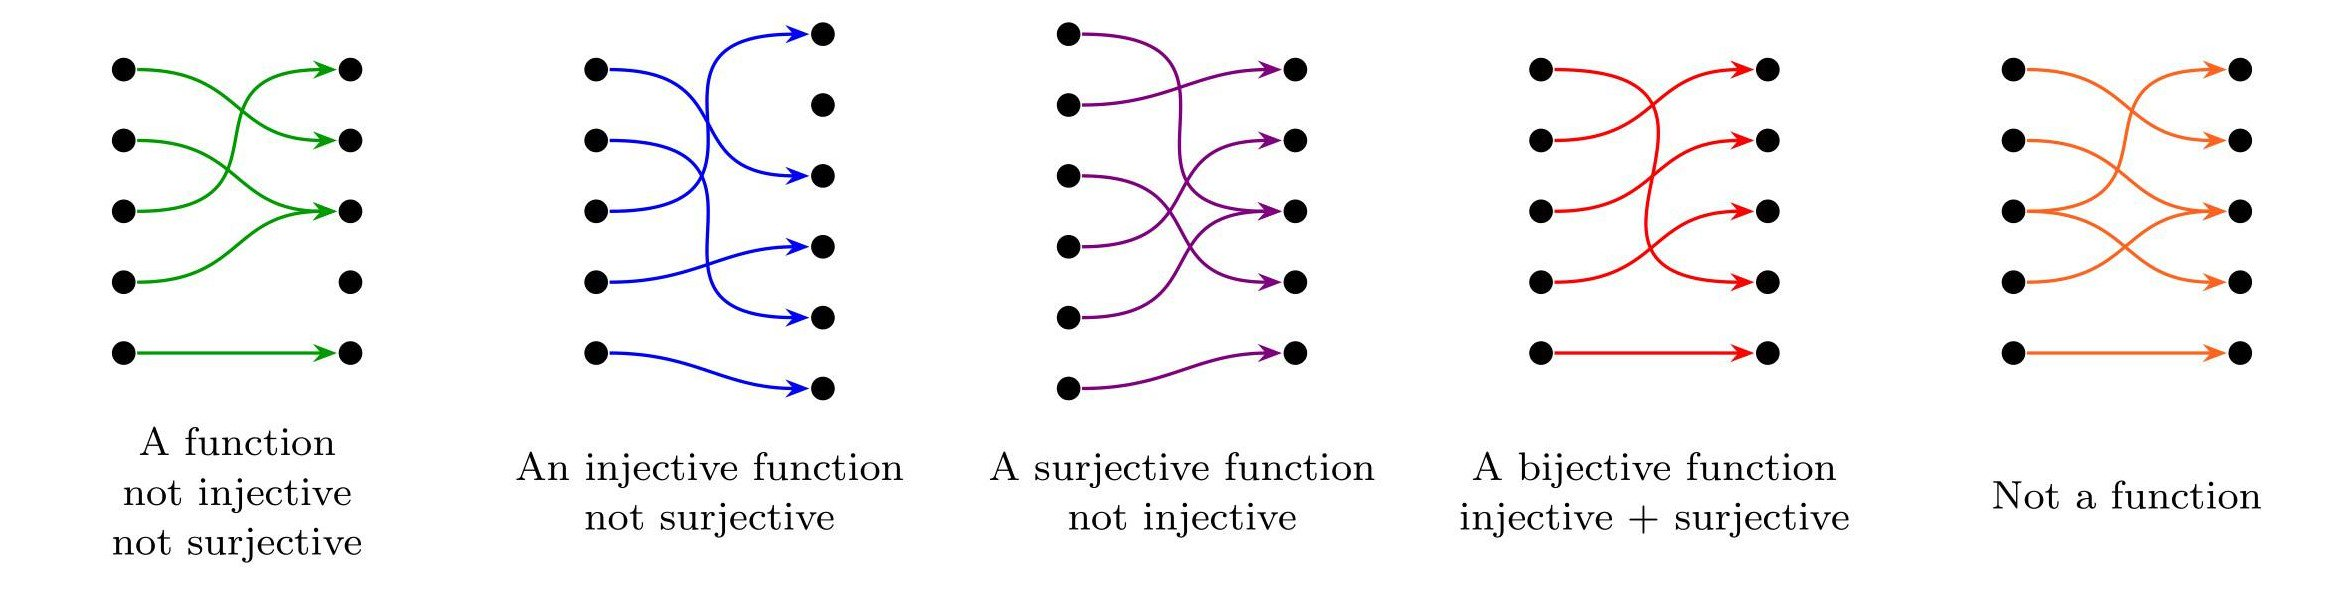
\includegraphics[width = 0.85\textwidth]{images/types-of-functions.jpeg}
            \end{itemize}
                \subsubsection*{Example.}
                    Let \( f: \mathbb{Z} \rightarrow \mathbb{N} \) be defined by \( f(x) = |x| + 1 \). Then \( f \) is surjective but not injective. The function \( f|_{\mathbb{N}} \) is injective but not surjective. Let \( \mathbb{Z}_{\geq 0} = \{ x \in \mathbb{Z} : x \geq 0 \} \). Then \( f|_{\mathbb{Z}_{\geq 0}} \) is both injective and surjective, hence a bijection. 
                \vspace*{0.5cm}
        %
        \item \textbf{Composition of functions:}\\ \\
            If \( f: S \rightarrow T \) and \( g: T \rightarrow U \) are functions, then the function which sends \( x \in S \) to \( g(f(x)) \) is the composite \( g \circ f: S \rightarrow U \), so \( g \circ f(x) = g(f(x)) \). \textcolor{red}{Remark: Even if \( f, g: S \rightarrow S \), we don’t necessarily have \( f \circ g = g \circ f \).} \\ \\
            \textbf{Exercise:} produce an example.\\
            \vspace*{0.5cm}
        \item \textbf{Inverse function:}\\ 
            Finally, a function \( f: S \rightarrow T \) is invertible if there exists a function \( g: T \rightarrow S \) such that
            \[
            g \circ f(x) = x \quad \forall x \in S, \quad \text{and} \quad f \circ g(y) = y \quad \forall y \in T.
            \]
            If it exists, such a \( g \) is the inverse of \( f \) and is denoted \( f^{-1} \).

            \textbf{Exercise.} Show that \( f \) is invertible iff it is bijective.

            \textbf{Example.} For the inverse of our function \( f: \mathbb{Z}_{\geq 0} \rightarrow \mathbb{N} \) from the last example is simply\\ \( f^{-1}(y) = y - 1 \).       
        \end{enumerate}
    
    

\newpage
\section*{Lecture 2: Fields ($\mathbb{F}$) \& Complex Numbers ($\mathbb{C}$) (Sep. $5^{th}$)}


\subsection*{\colorbox{yellow}{Fields $\mathbb{F}$}}
\qquad A field $F$ is a set equipped with two operations: 1. Addition $(+)$ \, 2. Multiplication $(\cdot)$\\
\qquad These operations satisfy that for each $x, y \in F$, there are unique elements $x + y \in F$ and $x \cdot y \in F$. Moreover, the following conditions hold:

\begin{enumerate}
    \item \textbf{Fields Axioms:}
            \begin{enumerate}
                \item \textbf{Commutativity of addition and multiplication:}
                    \[ a + b = b + a \quad \text{and} \quad a \cdot b = b \cdot a.\]
                
                \item \textbf{Associativity of addition and multiplication:}
                    \[(a + b) + c = a + (b + c) \quad \text{and} \quad (a \cdot b) \cdot c = a \cdot (b \cdot c).\]
                
                \item \textbf{Existence of identity elements:} There exist distinct elements $0$ and $1$ in $\mathbb{F}$ s.t.
                    \[ 0 + a = a \quad \text{(additive identity)}, \quad 1 \cdot a = a \quad \text{(multiplicative identity)}.\]
                
                \item \textbf{Existence of inverses:} $\forall a \in\mathbb{F}$ and each nonzero $b \in \mathbb{F}$, there exist $c, d \in \mathbb{F}$ s.t.
                    \[a + c = 0 \quad \text{and} \quad b \cdot d = 1.\]
                
                \item \textbf{Distributivity:}
                    \[a \cdot (b + c) = a \cdot b + a \cdot c.\]
            \end{enumerate}

        \subsubsection*{Examples of Fields}
            \begin{enumerate}
                \item $\mathbb{R}$, with usual $+$ and $\cdot$
                \item $\mathbb{Q}$, with usual $+$ and $\cdot$
                \item $\mathbb{Q}(\sqrt{5}) = \{x \in \mathbb{R} : x = a + b\sqrt{5} \text{ for } a, b \in \mathbb{Q} \}$
                \item $F_2 = \{0, 1\}$ with the operations:
                    \[0 + 0 = 0, \quad 0 + 1 = 1, \quad 1 + 1 = 0,\]
                    \[0 \cdot 0 = 0, \quad 0 \cdot 1 = 0, \quad 1 \cdot 1 = 1.\]
            \end{enumerate}

    \item \textbf{Properties of Fields}\\ \\
        \textbf{Theorem:} Let $F$ be a field and $a, b, c \in F$. Then:
        \begin{enumerate}
            \item If $c \neq 0$ and $a \cdot c = b \cdot c$, then $a = b$.
            \item If $a + c = b + c$, then $a = b$.
        \end{enumerate}

        \textbf{Proof of (1):} Let $d \in F$ be an element such that $c \cdot d = 1$ (by the existence of inverses, since $c \neq 0$). Then,
        \[
            (a \cdot c) \cdot d = (b \cdot c) \cdot d.
        \]
        By the associativity of multiplication,
        \[
            a \cdot (c \cdot d) = b \cdot (c \cdot d).
        \]
        Since $c \cdot d = 1$,
        \[
            a \cdot 1 = b \cdot 1.
        \]
        By the identity property,
        \[
            a = b.
        \]
        \textbf{Corollary:} The elements $0$ and $1$ (the identity elements), as well as the elements $c$ and $d$ (the inverses), are unique.
    \end{enumerate}

\subsection*{\colorbox{yellow}{Complex Numbers $\mathbb{C}$}}
    \begin{enumerate}
        \item \textbf{Definition:} The set of complex numbers is
        \[ \mathbb{C} = \{a + bi : a, b \in \mathbb{R}\}. \]
        
        \item \textbf{Operations:}
        \begin{itemize}
            \item \textbf{Addition:} $(a + bi) + (c + di) = (a + c) + (b + d)i$.
            \item \textbf{Multiplication:} $(a + bi) \cdot (c + di) = (ac - bd) + (ad + bc)i$.
        \end{itemize}
        
        \item \textbf{Example:} 
        \[
            (2 + i) \cdot (3 - 4i) = (2 \cdot 3 - (1 \cdot -4)) + i(2 \cdot -4 + 1 \cdot 3) = 10 - 5i.
        \]

        \item \textbf{Remark:} $\mathbb{R}$ is naturally a subset of $\mathbb{C}$, consisting of elements of the form $a + 0i$.
        
        \item \textbf{Imaginary numbers:} Numbers of the form $0 + bi$ are called \textbf{imaginary}. The product of two imaginary numbers is real:
        \[
            (0 + bi) \cdot (0 + ci) = -bc.
        \]

        \item \textbf{Complex conjugate:} For $z = a + bi$, the complex conjugate of $z$ is $\overline{z} = a - bi$. The modulus of $z$ is $|z| = \sqrt{a^2 + b^2}$. The inverse of $z$ is given by
        \[
            z^{-1} = \frac{\overline{z}}{|z|^2}.
        \]

        \item \textbf{Conclusion:} The complex numbers $\mathbb{C}$ form a field.
    \end{enumerate}
\newpage
\section*{Lecture 3: Modular Arithmetics (Sep. $10^{th}$)}


\subsection*{Last lecture: $\mathbb{F}$}
\qquad Recall \( \mathbb{F}_2 = \{0, 1\} \) with the following operations, and check if \( \mathbb{F}_2 \) is a field.:
    \[\begin{aligned}
        0 + 0 &= 0 \quad & 0 \cdot 0 &= 0 \\
        0 + 1 &= 1 \quad & 0 \cdot 1 &= 0 \\
        1 + 0 &= 1 \quad & 1 \cdot 0 &= 0 \\
        1 + 1 &= 0 \quad & 1 \cdot 1 &= 1 
    \end{aligned}\]


% Modular Arithmetic
\subsection*{\colorbox{yellow}{\#Modular Arithmetic.}}
    \qquad Let \( m \in \mathbb{N} \) and let \( a, b \in \mathbb{Z} \). We say \( a \) is congruent to \( b \) modulo (or mod) \( m \)\, if \, \(m \mid a - b\), and we denote that:
    \[\boldsymbol{a \equiv b \;\, \textbf{mod} \;\, m} \quad \text{or} \quad \boldsymbol{a \equiv b \, (m)}\]

\vspace*{0.2cm}

    \,\,\,\textbf{Example:} Let \( a = 3 \) and \( b = 45 \). Any of the following holds?:
        \[\begin{aligned}
            3 \equiv 45 \,\,(2) \quad \checkmark  \implies 2 \mid 3 - 45 \quad \checkmark\\ 
            3 \equiv 45 \,\,(3) \quad \checkmark  \implies 3 \mid 3 - 45 \quad \checkmark\\
            3 \equiv 45 \,\,(4) \quad \times \implies 4 \mid 3 - 45 \quad \times\\
            3 \equiv 45 \,\,(5) \quad \times \implies 5 \mid 3 - 45 \quad \times
        \end{aligned}\]
        \qquad \qquad  Question: Are there numbers \( m > 5 \) such that \( a \equiv b \pmod{m} \)?\\
        
        \qquad \textbf{Exercise:} Write down two numbers that are congruent modulo 5 but not congruent modulo 3.\\
        
        \qquad \textbf{Homework:} Show that being congruent modulo \( m \) is an equivalence relation on \( \mathbb{Z} \).
        
        
        %lemma
        \subsubsection{\colorbox{pink}{Lemma:}} 
        Let \( m \in \mathbb{N} \) and \( a, b \in \mathbb{Z} \), then \( a \equiv b \pmod{m} \iff \exists k \in \mathbb{Z} \text{ such that } a = b + mk.\) \newline
            \begin{minipage}[t]{1\textwidth}
                \vspace*{0.1cm}
                \begin{proof} 
                    \(\implies\)Suppose \( a \equiv b \pmod{m} \), then by definition, \( m \mid (a - b) \). This means that \( a - b \) is a multiple of \( m \), so it can be written as \( a - b = mk \) for some \( k \in \mathbb{Z} \). Rearranging, we get \( a = b + mk \), as claimed.
                    \(\impliedby\)Conversely, suppose \( a = b + mk \). Then \( a - b = mk \), which is divisible by \( m \). By definition, \( a \equiv b \pmod{m} \).
                \end{proof}
            \end{minipage}
            
            
        %Theorems
        \subsubsection{\colorbox{red}{Theorem}}
        Let \( m \in \mathbb{N},\, \forall a \in \mathbb{Z} \), there exists a \textbf{unique} \( r \in \{0, 1, \dots, m-1\} \) s.t. \( a \equiv r \pmod{m} \).\newline
            \begin{minipage}[t]{1\textwidth}
                \vspace*{0.1cm}
                \begin{proof}
                    We will show that there exist unique integers \( r, k \) such that \( a = r + km \) and \( 0 \leq r < m \). By the lemma, \( a \equiv r \pmod{m} \). \newline
                    \newline
                    \textbf{Existence:} Consider all integer multiples of \( m \), \( \{0, \pm m, \pm 2m, \dots \} \). These integers are equally spaced along the real line. The integer \( a \) lies somewhere on the real line in one of these intervals, i.e., it satisfies \( km \leq a < (k+1)m \) for some value of \( k \).
                    If we subtract \( km \) from this inequality, we find \( 0 \leq a - km < m \). Let \( r = a - km \), then \( r \) satisfies the desired conditions.\newline
                    \newline
                    \textbf{Uniqueness:} Suppose that \( a = r + km = r' + k'm \) with \( 0 \leq r, r' < m \). Then \(r + km = r' + k'm\) \(\implies r - r' = (k' - k)m.\) \,It follows that \( r - r' \) is a multiple of \( m \). But since \( 0 \leq r, r' < m \), we must have \( -m < r - r' < m \). The only multiple of \( m \) in that interval is zero, so \( r = r' \) and \( k = k' \).
                \end{proof}
            \end{minipage}
        
\newpage
        \subsubsection*{``Partitioning $\mathbb{Z}$ into  m  Congruence Classes" $\thicksim$ ``Congruence mod m"}
            \qquad We will call $\boldsymbol{\{0,1,2,3,4,5,\ldots,m-1\}}$ the standard representatives for the integers modulo $m$.\\
                \[\begin{aligned}
                    &\text{Let } m = 3, \text{ we have the following standard representatives that partition } \mathbb{Z}: \\
                    &\qquad \qquad  \overline{0} = \{ \ldots, -9, -6, -3, 0, 3, 6, 9, \ldots \} \\
                    &\qquad \qquad \overline{1} = \{ \ldots, -10, -7, -4, 1, 4, 7, 10, \ldots \} \\
                    &\qquad \qquad \overline{2} = \{ \ldots, -11, -8, -5, 2, 5, 8, 11, \ldots \}
                \end{aligned}\]
            \newline
                We define addition and multiplication with integers modulo m.






% Theorem: Field
\subsection*{\colorbox{yellow}{Theorem.}}
\( \mathbb{Z}/m\mathbb{Z} \) is a field if and only if \( m \) is a prime number.

\textbf{Proof:} Suppose \( m \) is not a prime number. Then there exist \( r, s \in \mathbb{Z} \) such that \( 0 < r, s < m \) and \( r \cdot s = m \). This implies that \( r \cdot s \equiv 0 \pmod{m} \), but \( r \neq 0 \) and \( s \neq 0 \). Therefore, \( \mathbb{Z}/m\mathbb{Z} \) contains zero divisors and hence is not a field.

Assume now that \( m \) is prime. We will use the following property of prime numbers: 
\[
\text{If } p \text{ is prime and } p \mid (x \cdot y), \text{ then either } p \mid x \text{ or } p \mid y.
\]
This property ensures that \( \mathbb{Z}/m\mathbb{Z} \) contains no zero divisors, and hence every non-zero element has a multiplicative inverse. Therefore, \( \mathbb{Z}/m\mathbb{Z} \) is a field. \(\square\)


% Claim
\subsection*{\colorbox{yellow}{Claim.}}
Let \( x \in \mathbb{Z}/m\mathbb{Z} \) and \( m \) be prime. Then if \( x \neq 0 \), the function
\[
f_x: \mathbb{Z}/m\mathbb{Z} \to \mathbb{Z}/m\mathbb{Z}, \quad y \mapsto xy
\]
is injective.

\textbf{Proof:} Let \( a, b \in \mathbb{Z}/m\mathbb{Z} \). Suppose \( a \equiv b \pmod{m} \), meaning \( m \mid (a - b) \). Fix a representative of \( x \) in \( \mathbb{Z} \), call it \( \tilde{x} \). Since \( x \neq 0 \), \( m \nmid \tilde{x} \).

Because \( m \) is prime, \( m \nmid \tilde{x}(a - b) \) by the property of prime numbers. Therefore, \( \tilde{x}a \not\equiv \tilde{x}b \pmod{m} \), i.e., \( xa \not\equiv xb \). This proves the claim. \(\square\)

% Surjectivity
\textbf{Surjectivity:} By HW1, Q1(b), the function is also surjective. That is, \( \forall s \in \mathbb{Z}/m\mathbb{Z}, \exists y \) such that \( xy = s \). In particular, there exists \( y \) such that \( xy = 1 \).

It follows that any element \( x \neq 0 \) has a multiplicative inverse. Therefore, if \( m \) is prime, \( \mathbb{Z}/m\mathbb{Z} \) is a field. \(\square\)

% Notation
\subsection*{\colorbox{yellow}{Notation.}}
We will denote prime numbers by \( p \), and we will often denote \( \mathbb{Z}/p\mathbb{Z} \) as \( \mathbb{F}_p \), the field with \( p \) elements.

% Modular Arithmetic Extended
\subsection*{\colorbox{yellow}{Modular Arithmetic.}}

\textbf{Definition:} The integers modulo \( m \), denoted \( \mathbb{Z}/m\mathbb{Z} \), is the set of congruence classes modulo \( m \). We will often denote the classes by their standard representatives, so we write:
\[
\mathbb{Z}/m\mathbb{Z} = \{0, 1, \dots, m-1\}.
\]

Thanks to the last theorem, \( \mathbb{Z}/m\mathbb{Z} \) is equipped with well-defined notions of addition and multiplication.

\textbf{Example:} \( \mathbb{Z}/3\mathbb{Z} = \{0, 1, 2\} \)
\[
\begin{aligned}
    0 + 0 &= 0 \quad & 0 + 1 &= 1 \quad & 0 + 2 &= 2 \\
    1 + 1 &= 2 \quad & 1 + 2 &= 0 \quad & 2 + 2 &= 1
\end{aligned}
\]

\textbf{Exercise:} Write the multiplication table for \( \mathbb{Z}/3\mathbb{Z} \).

Modular arithmetic is like arithmetic on a clock, except that the modulus \( m \) need not be 12, and multiplication is defined.

\textbf{Exercise:} Show that \( \mathbb{Z}/m\mathbb{Z} \), equipped with the operations \( + \) and \( \cdot \), satisfies the field axioms \( (F1), (F2), (F3), (F5) \) if \( m > 1 \).

% Existence of Inverses (Axiom F4)
\subsection*{\colorbox{yellow}{Existence of Inverses (Axiom F4).}}

\textbf{Exercise:} Prove that for every element \( a \in \mathbb{Z}/m\mathbb{Z} \), the class \( m - a \) is the additive inverse of the class of \( a \).

For the existence of multiplicative inverses, consider \( m = 4 \):
\[
\mathbb{Z}/4\mathbb{Z} = \{0, 1, 2, 3\}.
\]
Let's examine the element 2:
\[
\begin{aligned}
    2 \cdot 0 &= 0 \\
    2 \cdot 1 &= 2 \\
    2 \cdot 2 &= 0 \\
    2 \cdot 3 &= 2
\end{aligned}
\]
There is no \( x \in \mathbb{Z}/4\mathbb{Z} \) such that \( x \cdot 2 = 1 \). Therefore, \( \mathbb{Z}/4\mathbb{Z} \) fails Axiom (F4) and is not a field.

% Theorem: Field iff Prime
\subsection*{\colorbox{yellow}{Theorem: Field iff Prime.}}

\( \mathbb{Z}/m\mathbb{Z} \) is a field if and only if \( m \) is a prime number.

\textbf{Proof:} Suppose \( m \) is not a prime number. Then there exist \( r, s \in \mathbb{Z} \) such that \( 0 < r, s < m \) and \( r \cdot s = m \). This implies that \( r \cdot s \equiv 0 \pmod{m} \), but \( r \neq 0 \) and \( s \neq 0 \), so \( \mathbb{Z}/m\mathbb{Z} \) is not a field.

Assume now that \( m \) is prime. We will use the following property of prime numbers: 
\[
\text{If } p \mid (x \cdot y) \text{ and } p \text{ is prime}, \text{ then } p \mid x \text{ or } p \mid y.
\]
Because \( m \) is prime, this property ensures that \( \mathbb{Z}/m\mathbb{Z} \) contains no zero divisors. Since every non-zero element has a multiplicative inverse, \( \mathbb{Z}/m\mathbb{Z} \) is a field. \(\square\)


\end{document}